%%%%%%%%%%%%%%%%%%% Figure 2 %%%%%%%%%%%%%%%%%%%
\usetikzlibrary{datavisualization.formats.functions}
\begin{figure}[h!]
	\centering
	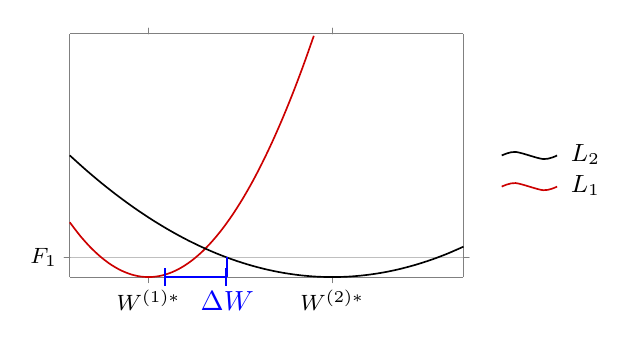
\begin{tikzpicture}[baseline]
		\datavisualization [
		scientific axes, 
		x axis = {ticks={major at={-0.2 as $W^{(1)*}$, 0.5 as $W^{(2)*}$}}},
		y axis = {max value = 0.2, ticks and grid ={major at={0.016 as $F_1$}}},
		visualize as smooth line/.list={w1,w2},
		style sheet=strong colors,
		w1 = {label in legend = {text=$L_2$}},
		w2 = {label in legend = {text=$L_1$}},
		data/format=function
		]
		data [set=w1] {
			var x : interval [-0.5:1];
			func y = 0.1 * (\value x - 0.5) * (\value x - 0.5);
		}
		data [set=w2] {
			var x : interval [-0.5:0.43];
			func y = 0.5 * (\value x  + 0.2) * (\value x + 0.2);
		};
		\usetikzlibrary{arrows.meta}
		\draw [thick, blue, |-|] (1.2, 0) -- (2, 0);
		\draw [thick, blue] (2, 0) -- (2, 0.25);
		\draw [blue] (2, -0.3) node {$\Delta W$};
	\end{tikzpicture}
	\caption{Depending on the curvature of $L_1$ and $L_2$, different $\Delta w$ result in different forgetting rates.}
	\label{fig:02}
\end{figure}